\subsection{Event study around mobile takeoff (A4b)}
The first event-study design, stacked cohorts with controls that adopt more than ten years later or never, was not interpretable (Section~\ref{sec:methods}, Appendix~\ref{app:amend}): nearly every economy crosses the threshold in the window, only 7 clean controls existed for the low and lower-middle income group, and that group showed a pre-trend of 12 log points. The replacement design compares each cohort with economies not yet treated at each horizon and adjusts for initial income and earlier growth. It passes the pre-trend rule in all four samples when the takeoff threshold is 10 subscriptions per 100 (mean placebo effect between $-0.9$ and $0.6$ log points, all intervals including zero; Table~\ref{tab:event}).

\begin{table}[ht]\centering\small
\caption{Event study around the year mobile subscriptions reach 10 per 100 people: effect on log GDP per capita ($\times100$) relative to the year before takeoff and to economies not yet treated (95\% bootstrap interval, 400 draws). Pre-trend: mean of the placebo effects at $-5$ to $-2$ years.}\label{tab:event}
\begin{tabular}{@{}lrlll@{}}\toprule
Sample & Treated & Pre-trend & Effect at +5 years & Effect at +10 years\\\midrule
All economies & 178 & $-0.0$ [$-0.6$, 0.4] & 13.5 [0.6, 36.5] & 47.8 [$-12.5$, 149.1]\\
Low and lower-middle & 66 & 0.6 [$-0.6$, 1.6] & $-5.9$ [$-18.6$, 31.9] & not estimable\\
Upper-middle & 56 & $-0.9$ [$-2.0$, 0.3] & 11.9 [$-8.0$, 46.7] & 12.2 [$-70.1$, 118.6]\\
High & 56 & $-0.4$ [$-1.2$, 0.5] & 19.1 [6.2, 36.7] & 53.8 [4.2, 152.6]\\\bottomrule
\end{tabular}\end{table}

\begin{figure}[ht]\centering
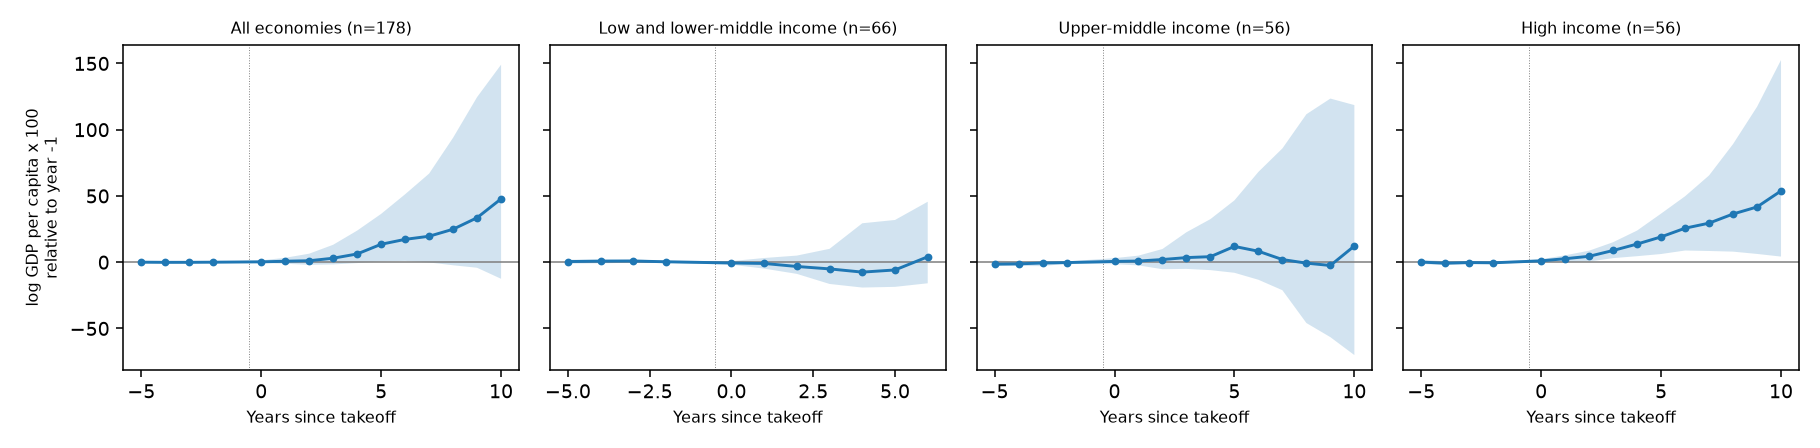
\includegraphics[width=\textwidth]{fig_event.png}
\caption{Event-study estimates by income group (takeoff at 10 mobile subscriptions per 100; shaded: 95\% bootstrap interval). The low and lower-middle panel stops at six years because fewer than eight not-yet-treated economies exist at longer horizons.}\label{fig:event}
\end{figure}

Economies that reach 10 subscriptions per 100 earlier have higher GDP per capita five years later than comparable economies that reach it later, by about 14 log points (95\% CI 0.6 to 36.5). The difference is distinguishable from zero only for high-income economies (19 log points, CI 6.2 to 36.7); the interval for low and lower-middle income economies, $-18.6$ to $+31.9$, is wide enough to contain effects of either sign and of the high-income size. Magnitudes at ten years (about 48 log points overall) are implausibly large for an effect of mobile telephony alone. They mainly show that economies reaching the threshold early are on different growth paths from those reaching it later, in ways initial income and earlier growth do not capture, and that at long horizons only the earliest cohorts contribute. The results are similar with a threshold of 25 per 100 (high income: 15.7 at five years, CI 6.5 to 28.8; low and lower-middle: $-7.5$, CI $-17.6$ to 13.3). With a threshold of 50, the pooled sample and the upper-middle sample fail the pre-trend rule and are not interpreted; the low and lower-middle estimate is 4.3 (CI $-10.7$ to 13.9) and the high-income estimate 8.9 (CI $-0.8$ to 20.8) (Appendix Tables~\ref{tab:es25} and~\ref{tab:es50}).

\emph{Outcomes beyond income.} For samples that pass the pre-trend rule, life expectancy is about 0.9 years higher five years after takeoff in the pooled sample (CI 0.1 to 1.7) and 0.8 years in high-income economies (CI 0.0 to 1.5), with a larger but imprecise estimate for low and lower-middle income economies (2.6 years, CI $-0.5$ to 6.4). Under-5 mortality is 15 log points lower in low and lower-middle income economies (CI $-26.0$ to 1.0). Unemployment and the agriculture share fail the pre-trend rule in most samples, and electricity use is not distinguishable from zero (Appendix Table~\ref{tab:essec}). These outcomes have strong secular trends, so we read these as descriptive.

\subsection{Local projections (A7)}
Local projections give a dynamic profile without a binary treatment (Table~\ref{tab:lp}, Figure~\ref{fig:lp}). For lower-middle income economies, a 10-subscription increase over three years is followed by cumulative growth that is higher by 0.41 percentage points after one year and by 2.0 points after six years (CI 0.8 to 3.2), then 1.7 after eight. For upper-middle and high-income economies, the profile is flat, and the high-income point estimate turns slightly negative (cumulative $-0.5$ after eight years, CI $-1.2$ to 0.2). For low-income economies the profile starts positive and turns negative ($-4.3$ after eight years, CI $-9.2$ to 0.6), but the intervals include zero except as noted. The placebo (future adoption against past growth) is close to zero in every group, though with a wide interval for low-income economies ($-0.75$, CI $-2.5$ to 1.0).

\begin{table}[ht]\centering\small
\caption{Local projections: cumulative growth of GDP per capita (percentage points) $h$ years after a +10 change in mobile subscriptions per 100 over the previous three years (95\% CI; country and year fixed effects).}\label{tab:lp}
\begin{tabular}{@{}lrllll@{}}\toprule
Group & Economies & $h=1$ & $h=2$ & $h=4$ & $h=8$\\\midrule
Low & 24 & 0.25 [$-0.08$, 0.58] & 0.34 [$-0.35$, 1.04] & $-0.44$ [$-2.23$, 1.35] & $-4.31$ [$-9.19$, 0.57]\\
Lower-middle & 47 & 0.41 [0.11, 0.71] & 0.76 [0.25, 1.27] & 1.51 [0.69, 2.33] & 1.69 [0.32, 3.07]\\
Upper-middle & 58 & $-0.00$ [$-0.21$, 0.21] & 0.10 [$-0.19$, 0.38] & 0.22 [$-0.45$, 0.88] & 0.17 [$-0.99$, 1.34]\\
High & 74 & 0.08 [$-0.04$, 0.19] & 0.06 [$-0.16$, 0.29] & $-0.06$ [$-0.48$, 0.35] & $-0.51$ [$-1.23$, 0.20]\\\bottomrule
\end{tabular}\end{table}

\begin{figure}[ht]\centering
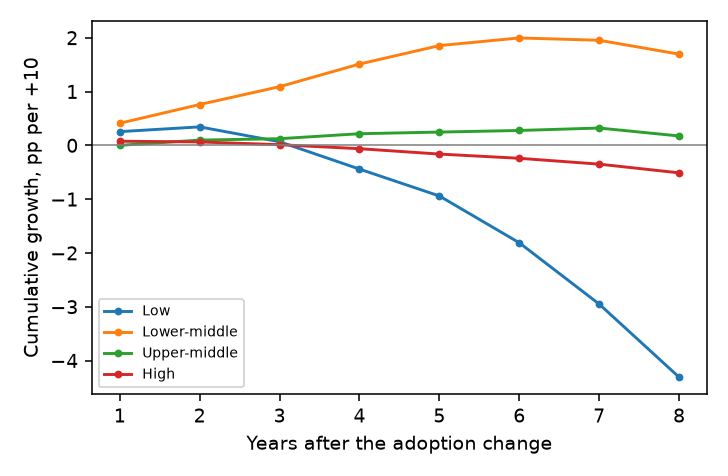
\includegraphics[width=0.6\textwidth]{fig_lp.png}
\caption{Local-projection profiles by income group.}\label{fig:lp}
\end{figure}

\subsection{Consistency across designs}
Table~\ref{tab:designs} summarises which income group shows a positive association under each design. No group is positive under all four. Lower-middle income economies are positive under three (A1, A2, local projections); under the event study they are pooled with low-income economies and the pooled estimate is null with a negative point estimate. High-income economies are positive under the same-period regression and the event study, but flat or negative under the predetermined regression and the local projections. Upper-middle economies are positive only in the same-period regression. Low-income economies are never significantly positive. We conclude that the panel analysis does not support a statement that richer or poorer economies gain more; the answer depends on the design, which is the same message as in the reviewed studies.

\begin{table}[ht]\centering\small
\caption{Direction and significance of the association between mobile adoption and GDP per capita growth, by design and income group (+ positive and significant at 5\%, $-$ negative and significant, 0 not significant; sign of the point estimate in parentheses).}\label{tab:designs}
\begin{tabular}{@{}lllll@{}}\toprule
Design & Low & Lower-middle & Upper-middle & High\\\midrule
A1 same period & 0 (+) & + & + & +\\
A2 previous period & 0 ($-$) & + & 0 (+) & $-$\\
Event study (+5 years) & \multicolumn{2}{c}{0 ($-$), low and lower-middle pooled} & 0 (+) & +\\
Local projections ($h=6$) & 0 ($-$) & + & 0 (+) & 0 ($-$)\\\bottomrule
\end{tabular}\end{table}
